\documentclass{article}
\usepackage{longtable}
\usepackage{multirow}
\usepackage{array}
\usepackage{graphicx}  % For inserting images
\usepackage{caption}   % For better caption formatting
\usepackage{float}     % To control figure placement


\title{Open Science Platform Artifact}
\author{Eduardo Oliveira}
\date{\today}

\begin{document}

\maketitle

\section{Open Science Platform}

\subsection{Overview}

The Open Science platform aims to empower researchers and members of the scientific community by providing a secure, transparent, traceable and tamper-proof environment for sharing project artifacts and data. Building on this objective, the platform leverages decentralized technologies to ensure the integrity and reliability of shared information.


\subsection{Technology Stack}

The Open Science platform is built upon a robust technical foundation, comprising:

\begin{itemize}
    \item Hyperledger Iroha v1 Blockchain: The core infrastructure for account management and transaction recording and business rules enforcement through Smart Contracts ensuring secure and transparent data exchange.
    \item IPFS (InterPlanetary File System): The decentralized storage for project artifacts and metadata, guaranteeing tamper-proof and persistent access to shared information.
\end{itemize}


Aside from the decentralized technologies above, the platform also relies on the following off-chain, centralized components:

\begin{itemize}
    \item Jupyter Notebooks in Python: The front-end interface of the platform leverages Jupyter Notebooks in Python to automate and display the execution steps of the activities in the platform.
    \item Apache Tika: Utilized for extracting file metadata, enhancing the platform's ability to manage and describe artifact content.
    \item Woosh: For efficient indexing and search capabilities for artifacts stored on the platform.
\end{itemize}

\subsection{Operations}



\vspace{1cm}

\begin{figure}[H]
    \centering
    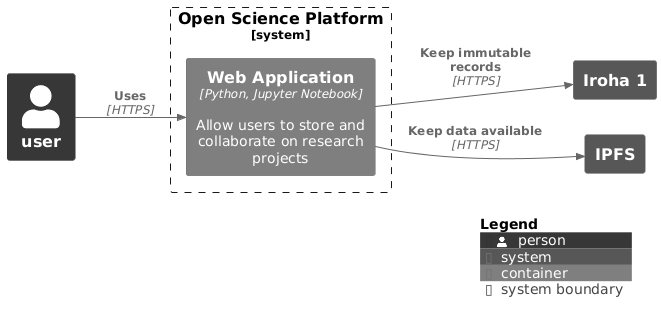
\includegraphics[width=\textwidth]{/home/eduardo/Documents/repo/Git/OpenScience/out/diagrams/plantUML/system_diagram/system_diagram.png}  % Placeholder for the SVG file
    \caption{System diagram for the Open Science Platform.}
    \label{fig:system-diagram}
\end{figure}


\vspace{1cm}

\begin{figure}[H]
    \centering
    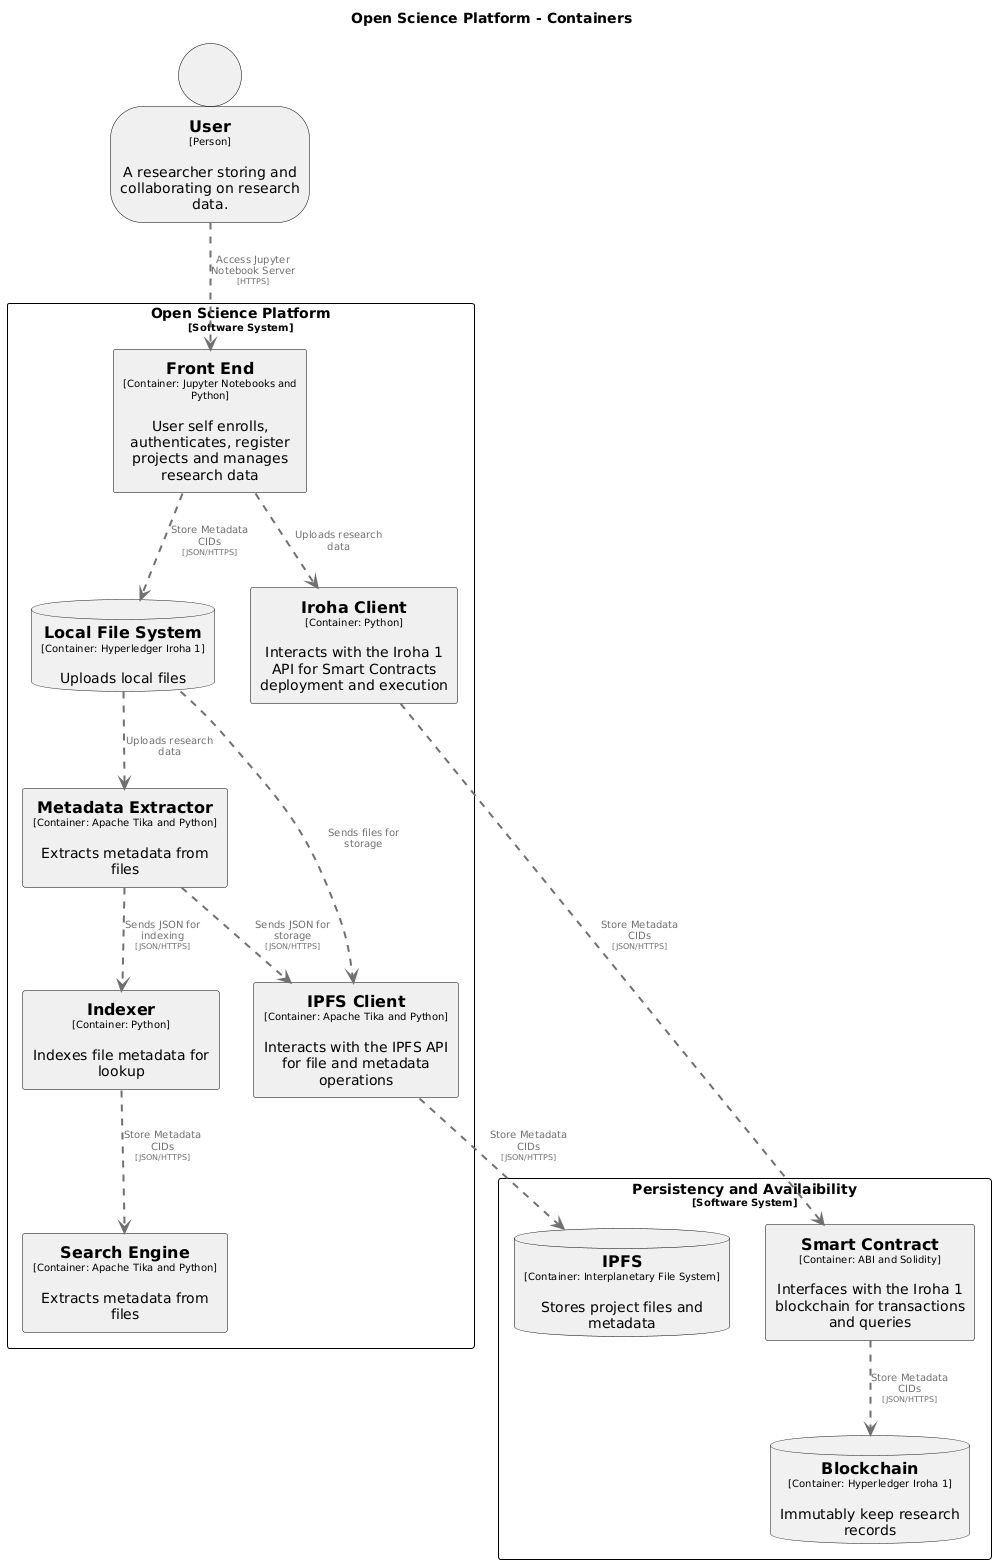
\includegraphics[width=\textwidth]{/home/eduardo/Documents/repo/Git/OpenScience/out/diagrams/plantUML/container_diagram/container_diagram.png}  % Placeholder for the SVG file
    \caption{System diagram for the Open Science Platform.}
    \label{fig:container-diagram}
\end{figure}


\subsection{Operations}


\begin{longtable}{|l|l|p{8cm}|}
    \hline
    \multicolumn{1}{|c|}{\textbf{Entity}}   &
    \multicolumn{1}{c|}{\textbf{Attribute}} &
    \multicolumn{1}{c|}{\textbf{Description}}                                                                                           \\
    \hline
    \multirow{2}{*}{\texttt{foaf:Person}}
                                            & foaf:name         & The name of the person.                                               \\ \cline{2-3}
                                            & foaf:mbox         & The email address of the person.                                      \\ \cline{2-3}
    \hline
    \multirow{3}{*}{\texttt{foaf:holdsAccount}}
                                            & schema:identifier & The account name of the person in the blockchain.                     \\ \cline{2-3}
                                            & schema:roleName   & The role of the person in the platform.                               \\ \cline{2-3}
                                            & schema:publicKey  & The cryptographic public key of the account in the blockchain.        \\
    \hline
    \multirow{1}{*}{\texttt{foaf:Organization}}
                                            & foaf:name         & The name of the organization the person belongs to.                   \\ \cline{1-3}

    \hline
    \multirow{2}{*}{\texttt{schema:identifier}}
                                            & propertyID        & The type of identifier is ORCID (Open Researcher and Contributor ID). \\ \cline{2-3}
                                            & value             & The actual ORCID value for the person.                                \\
    \hline
\end{longtable}

\subsection{Project Account}

\begin{longtable}{|l|l|p{8cm}|}
    \hline
    \multicolumn{1}{|c|}{\textbf{Entity}}   &
    \multicolumn{1}{c|}{\textbf{Attribute}} &
    \multicolumn{1}{c|}{\textbf{Description}}                                                                           \\
    \hline
    \multirow{3}{*}{\texttt{foaf:Person}}
                                            & foaf:name         & The name of the person.                               \\ \cline{2-3}
                                            & foaf:mbox         & The email address of the person.                      \\ \cline{2-3}
                                            & foaf:holdsAccount & Links the person to an account.                       \\
    \hline
    \multirow{2}{*}{\texttt{foaf:Organization}}
                                            & foaf:name         & The name of the organization.                         \\ \cline{2-3}
                                            & foaf:location     & The physical or digital location of the organization. \\
    \hline
    \multirow{2}{*}{\texttt{schema:identifier}}
                                            & propertyID        & The type of identifier (e.g., ORCID).                 \\ \cline{2-3}
                                            & value             & The actual identifier value.                          \\
    \hline
\end{longtable}


\section{Entity-Relationship Diagram}

The diagram below represents the relationships between various entities extracted from the given JSON-LD data. The main entities in the diagram include:

\begin{itemize}
    \item \textbf{foaf:Person} – Represents an individual, identified by attributes such as name, email, and affiliation.
    \item \textbf{foaf:Organization} – Represents an institution or organization to which a person is affiliated.
    \item \textbf{foaf:holdsAccount} – Represents an individual's digital account, containing an identifier, role, and public key.
    \item \textbf{schema:identifier} – Represents a unique identifier (such as an ORCID) assigned to a person.
\end{itemize}


\vspace{1cm}

\begin{figure}[H]
    \centering
    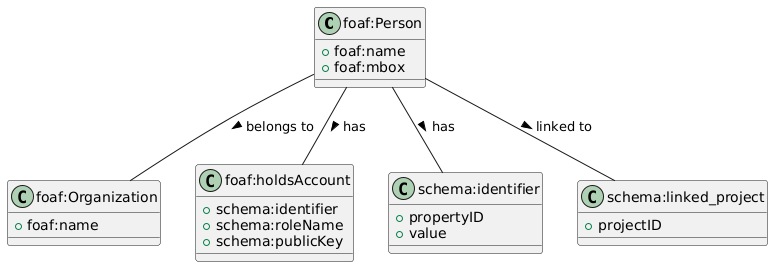
\includegraphics[width=\textwidth]{/home/eduardo/Documents/repo/Git/OpenScience/out/diagrams/plantUML/account/account.png}  % Placeholder for the SVG file
    \caption{Entity-Relationship diagram for the user account.}
    \label{fig:er-user-account-diagram}
\end{figure}


\vspace{1cm}

\begin{figure}[H]
    \centering
    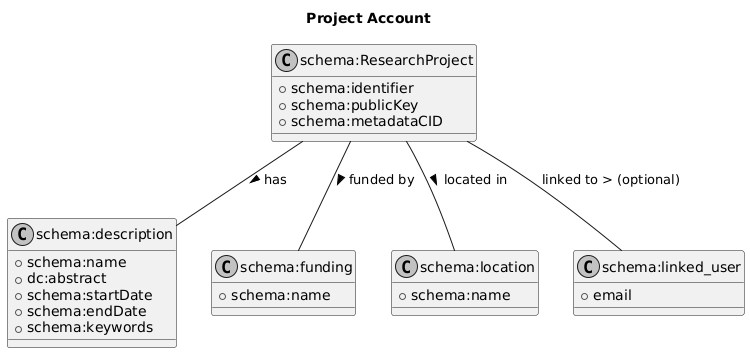
\includegraphics[width=\textwidth]{/home/eduardo/Documents/repo/Git/OpenScience/out/diagrams/plantUML/project/project.png}  % Placeholder for the SVG file
    \caption{Entity-Relationship diagram for the project account.}
    \label{fig:er-project-account-diagram}
\end{figure}



\end{document}


